\section{The Nested-CES Model}
\label{sec:nestedces}

We now give economic content to these two components in a nested-CES trade model.

\subsection{Production, preferences and equilibrium}
\label{sec:model}

Each country $i\in\{1,\dots,N\}$ is endowed with $L_i$ units of labor, its size, which is mobile across sectors. It produces a country-specific tradable and a non-tradable with labor only, $Y_{Ti}=A_{Ti}L_{Ti}$ and $Y_{Ni}=A_{Ni}L_{Ni}$, with $L_{Ti}+L_{Ni}=L_i$. Normalizing each tradable's producer price to one in its own currency, $w_i=A_{Ti}$ and $P_{Ni}=A_{Ti}/A_{Ni}$. Relative international producer prices therefore move only through exchange rates, and \textbf{the bilateral exchange rate equals the bilateral terms of trade and the relative wage in a common currency.}

Preferences are
\begin{equation}
C_i=C_{Ti}^{\alpha_T}C_{Ni}^{1-\alpha_T},\quad
C_{Ti}=\Big[\alpha_D^{1/\eta}C_{Tii}^{\frac{\eta-1}{\eta}}+(1-\alpha_D)^{1/\eta}M_i^{\frac{\eta-1}{\eta}}\Big]^{\frac{\eta}{\eta-1}},\quad
M_i=\Big[\textstyle\sum_{j\neq i}\beta_{ij}^{1/\rho}C_{Tji}^{\frac{\rho-1}{\rho}}\Big]^{\frac{\rho}{\rho-1}}.
\label{eq:prefs}
\end{equation}
Here $\eta$ governs substitution between domestic tradables and the import composite, and $\rho$ substitution across foreign origins; the latter is inactive when $N=2$. Country $i$ levies $\tau_{ij}$ on imports from $j$, so the consumer price is $p_{ij}=(1+\tau_{ij})e_{ij}$, and the import and tradable price indices are $P_{Mi}=[\sum_{j\neq i}\beta_{ij}p_{ij}^{1-\rho}]^{1/(1-\rho)}$ and $P_{Ti}=[\alpha_D+(1-\alpha_D)P_{Mi}^{1-\eta}]^{1/(1-\eta)}$. Tariff revenue is rebated lump-sum, so income is
\begin{equation}
I_i=\frac{w_iL_i}{1-\sum_{j\neq i}\frac{\tau_{ij}}{1+\tau_{ij}}s_{ij}},
\label{eq:income}
\end{equation}
with $s_{ij}$ the realized tariff-inclusive expenditure share of income on $j$'s good. Trade balances are measured at border prices,
\begin{equation}
\TB_i=\sum_{k\neq i}f_{ki}-\sum_{j\neq i}f_{ij},\qquad f_{ij}=\frac{s_{ij}\tilde I_i}{1+\tau_{ij}},
\label{eq:tb}
\end{equation}
with $\tilde I_i=e_{Ai}I_i$ income in $A$'s currency. Under the normalization $v_A=1$ of \cref{sec:bilateral}, values in $A$'s currency equal values in the common unit of account, so \cref{eq:tb} is the trade-balance measure of \cref{sec:framework}: flows at border prices, with tariff revenue a domestic transfer. The NEER is the one defined in \cref{sec:decomposition}, written here for any country $i$: $E_i=\prod_{j\neq i}e_{ij}^{w_{ij}}$ with baseline trade weights $w_{ij}=(f_{ij}+f_{ji})/\sum_{k\neq i}(f_{ik}+f_{ki})$; throughout, ``effective exchange rate'' refers to this trade-weighted NEER. The real exchange rate is $q_{ij}=e_{ij}P_j/P_i$, with $P_i$ the consumer price index.

The \textbf{symmetric benchmark} is free trade with $\beta_{ij}=1/(N-1)$, common parameters, and equal endowments and productivities. It retains home bias $\alpha_D$. Write $m\equiv\alpha_T(1-\alpha_D)$ for the import share of income.

\subsection{The two-country case}
\label{sec:twocountry}

With one foreign supplier, linearizing gives $d\TB_A=mM_2\,d\nu_B+m\rho_D\,d\tau$, so
\begin{equation}
\begin{gathered}
\frac{d\log e_{AB}}{d\tau}\bigg|_{\tau=0}=-\frac{\rho_D}{M_2},\\
\rho_D\equiv\underbrace{\alpha_D\eta}_{\text{domestic substitution}}+\underbrace{(1-\alpha_D)(1-\alpha_T)}_{\text{rebate / non-tradables}},\qquad
M_2\equiv1+2\alpha_D(\eta-1)=\varepsilon_X+\varepsilon_M-1.
\end{gathered}
\label{eq:twocountry}
\end{equation}
$\rho_D$ is the \textbf{domestic diversion margin}. It measures how strongly a tariff pulls expenditure toward the domestic economy, through substitution toward the domestic tradable and through the rebate's income effect on non-tradables. An exchange-rate movement generates no revenue, so it has no rebate term. This is why $\rho_D\neq M_2$.

\subsection{The \texorpdfstring{$N$}{N}-country case}
\label{sec:theorem}

We now evaluate the eigenvalues of \cref{sec:decomposition} in this model.

\begin{theorem}[Exchange-rate responses in the symmetric nested-CES model]
\label{thm:main}
At the symmetric benchmark define
\begin{equation}
M_N\equiv\frac{1}{N-1}\Big[\,1+\underbrace{N\alpha_D(\eta-1)}_{\text{domestic--import adjustment}}+\underbrace{(N-2)\rho}_{\text{foreign-origin adjustment}}\Big].
\label{eq:MN}
\end{equation}
The eigenvalues of \cref{prop:decomposition} are (\cref{lem:jacobian} and \cref{eq:geigen})
\begin{equation}
g_S=-\frac{m\rho_D}{N-1},\qquad g_D=-\frac{m\rho}{N-1},\qquad j_S=\frac{mM_N}{N-1},\qquad j_D=Nj_S.
\label{eq:eigenvalues}
\end{equation}
MML holds if and only if $M_N>0$, and $\eta\geq1$ suffices. When it holds,
\begin{equation}
\lambda_{\mathrm{avg}}=-\frac{\rho_D}{M_N},\qquad \lambda_{\mathrm{rel}}=-\frac{\rho}{NM_N},\qquad d\nu_j=\lambda_{\mathrm{avg}}\bar t+\lambda_{\mathrm{rel}}\widetilde t_j.
\label{eq:lambdas}
\end{equation}
\end{theorem}

$M_N$ measures how sensitive $A$'s trade balance with the rest of the world is to its effective exchange rate: $d\TB_A=mM_N\,d\nu^E_A$, with the equal weights of the symmetric benchmark. When $N>2$ it includes $\rho$, because foreign buyers can substitute between $A$'s goods and other foreign goods. For $N=2$ it reduces to $M_2$. Average protection works as in the two-country case. Relative treatment is zero-sum, so to first order it leaves revenue, income and the tradable/non-tradable split unchanged, and its disturbance is governed by $\rho$ alone.

The factor $1/N$ in $\lambda_{\mathrm{rel}}$ is central. A common exchange-rate move shifts only partners' trade with $A$. A relative move also shifts partners' trade with \emph{each other}. At the symmetric benchmark $A$ accounts for a share $1/N$ of the trade on which relative movements act, so $j_D=Nj_S$. \textbf{Relative exchange-rate adjustment is $N$ times as effective as common adjustment}, and a given relative disturbance requires only $1/N$ as much exchange-rate movement.

\subsection{A unilateral tariff}
\label{sec:unilateral}

\begin{figure}[t]
\centering
\begin{subfigure}[t]{0.45\textwidth}\centering
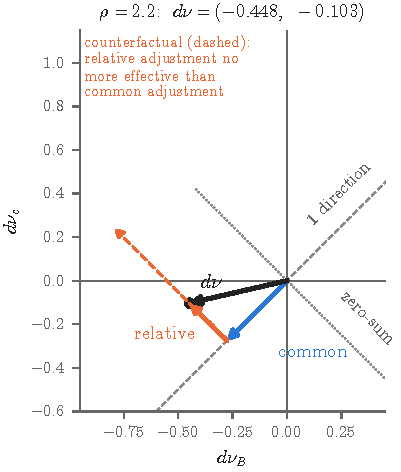
\includegraphics[width=\textwidth]{fig2a_geometry.pdf}
\caption{$\rho=2.2$: $\rho_D<\rho<3\rho_D$}
\label{fig:geometry-a}
\end{subfigure}\hfill
\begin{subfigure}[t]{0.45\textwidth}\centering
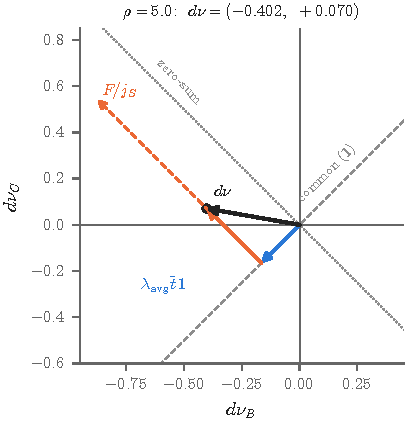
\includegraphics[width=\textwidth]{fig2b_geometry.pdf}
\caption{$\rho=5$: $\rho>3\rho_D$}
\label{fig:geometry-b}
\end{subfigure}
\caption{Average protection and relative treatment, $N=3$. A unilateral tariff on $B$, $t=(1,0)$, moves exchange rates through a common component (blue) and a relative component (solid orange); the black arrow is the equilibrium response $d\nu$, and the dashed arrow $F/j_S$ is the response if relative adjustment were no more effective than common adjustment. In (a), $C$'s trade balance improves at unchanged exchange rates, yet $A$ still appreciates against $C$. In (b), $A$ depreciates against $C$. The NEER appreciates in both. \textit{Notes:} $\alpha_D=0.7$, $\alpha_T=0.6$, $\eta=1.5$, so $\rho_D=1.17$ and $3\rho_D=3.51$.}
\label{fig:geometry}
\end{figure}

Let $A$ raise its tariff on $B$ alone, $t=d\tau\,e_B$. Then $\bar t=d\tau/(N-1)$, $\widetilde t_B=\frac{N-2}{N-1}d\tau$ and $\widetilde t_C=-\frac{d\tau}{N-1}$ for every bystander $C$.

\begin{proposition}[Unilateral tariff]
\label{prop:unilateral}
At the symmetric benchmark under MML,
\begin{equation}
\frac{d\nu^E_A}{d\tau}=-\frac{\rho_D}{(N-1)M_N}<0,\qquad
\frac{d\nu_B}{d\tau}=-\frac{N\rho_D+(N-2)\rho}{N(N-1)M_N}<0,\qquad
\frac{d\nu_C}{d\tau}=\frac{\rho-N\rho_D}{N(N-1)M_N}.
\label{eq:unilateral}
\end{equation}
\begin{enumerate}[label=(\roman*)]
\item $A$'s NEER appreciates for every $N$ and $\rho$.
\item $A$ appreciates against the target.
\item $A$ \textbf{depreciates against each untariffed bystander if and only if $\rho>N\rho_D$.}
\item The same threshold applies when $A$ tariffs any $k\leq N-2$ partners. More generally, $A$ depreciates against a partner $j$ facing a below-average tariff increase if and only if $t_j/\bar t<1-N\rho_D/\rho$, which requires $\rho>N\rho_D$.
\end{enumerate}
\end{proposition}

Against the target, average protection and relative treatment reinforce each other. Against a bystander they pull apart. Average protection shifts expenditure toward the domestic economy (appreciation), while the bystander's favorable relative treatment redirects expenditure toward it (depreciation).

\begin{corollary}[Why a single elasticity cannot deliver reversal]
\label{cor:single}
With home bias $\alpha_D\geq1/N$,
\begin{equation}
N\rho_D-\eta=\eta(N\alpha_D-1)+N(1-\alpha_D)(1-\alpha_T)\geq0,
\label{eq:single}
\end{equation}
so $\rho>\eta$ is \textbf{necessary} for a bystander depreciation. In any specification with a single elasticity across all tradable varieties ($\rho=\eta=\sigma$), $A$ appreciates against every bystander at every $\sigma$. At $\alpha_D=1/N$ the response is $-(1-\alpha_T)/(N\sigma)$, which approaches zero from below but never crosses it.
\end{corollary}

This explains why the natural first extension of the two-country model, a third country under a single CES elasticity, has not surfaced the reversal. The reversal requires that cross-origin substitution exceed home--import substitution, an ordering supported by the macro--micro elasticity evidence \citep{feenstra2018,li2022}. At US-like parameters ($\alpha_D=0.8$, $\alpha_T=0.4$, $\eta=1.5$, so $\rho_D=1.32$), $N\rho_D=3.96$ for $N=3$.

\paragraph{Disturbance versus equilibrium.} At unchanged exchange rates the bystander's trade balance improves if and only if $\rho>\rho_D$:
\begin{equation}
F_C=\frac{m(\rho-\rho_D)}{(N-1)^2}.
\label{eq:FC}
\end{equation}
The equilibrium bystander depreciation requires the stronger condition $\rho>N\rho_D$. The gap is the $1/N$ effectiveness of relative adjustment. For $\rho_D<\rho<N\rho_D$, $C$ gains at the old exchange rates yet ends up with a weaker currency against $A$ (\cref{fig:geometry-a}). \Cref{fig:unilateral} plots the three responses against $\rho$.

\begin{figure}[t]
\centering
\begin{subfigure}[t]{0.45\textwidth}\centering
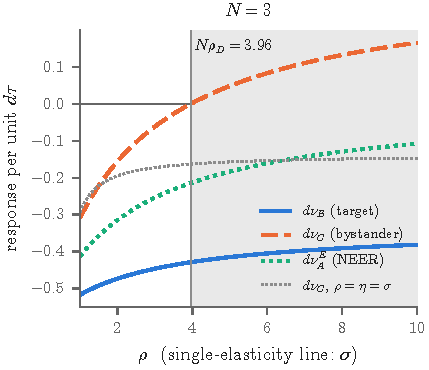
\includegraphics[width=\textwidth]{fig3a_unilateral.pdf}
\caption{$N=3$}
\end{subfigure}\hfill
\begin{subfigure}[t]{0.45\textwidth}\centering
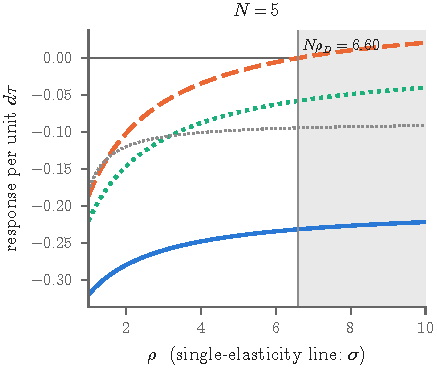
\includegraphics[width=\textwidth]{fig3b_unilateral.pdf}
\caption{$N=5$}
\end{subfigure}
\caption{Bilateral and effective responses to a unilateral tariff, per unit $d\tau$, US-like parameters ($\alpha_D=0.8$, $\alpha_T=0.4$, $\eta=1.5$). $d\nu_B$ and $d\nu^E_A$ are negative for every $\rho$; $d\nu_C$ crosses zero at $N\rho_D$ ($3.96$ for $N=3$, $6.60$ for $N=5$), and the shaded region is $\rho>N\rho_D$. The grey dotted line is the single-elasticity case $\rho=\eta=\sigma$, plotting $d\nu_C$ against $\sigma$; it never crosses zero (\cref{cor:single}). Closed forms of \cref{prop:unilateral}, verified against the linear solver.}
\label{fig:unilateral}
\end{figure}

\subsection{The three-country representation}
\label{sec:composite}

The $N$-country results can be read through a three-country economy, which we use as the workhorse for intuition. When the $N-2$ bystanders are symmetric and the tariff shock preserves that symmetry, no relative-price movement within the bystander bloc is activated. The bloc then has a single active direction, and the tariff experiment reduces exactly to three regions: $A$, $B$ and a composite bystander $C$. We now show that this composite is itself a nested-CES country, and we identify its parameters.

\begin{proposition}[Exact three-country reduction]
\label{prop:composite}
At the symmetric benchmark, consider any tariff change among $A$, $B$ and the bystanders that is common across bystanders: tariffs by $A$ or $B$ on all bystanders, by all bystanders on $A$ or $B$, or between $A$ and $B$. To first order, the responses of $\nu_B$, of every bystander rate $\nu_C$ and of $A$'s NEER coincide with those of a three-country nested-CES economy $\{A,B,C\}$ in which:
\begin{itemize}
\item $C$ has income $y_C=N-2$;
\item $A$ and $B$ place import weight $\frac{N-2}{N-1}$ on $C$ and $\frac{1}{N-1}$ on each other;
\item $C$ places import weight $\tfrac12$ on each of $A$ and $B$, with cross-origin elasticity $\rho$;
\item $C$'s home share of tradables is $h_C=\alpha_D+(1-\alpha_D)\frac{N-3}{N-1}$, equivalently $(N-1)h_C=N-3+2\alpha_D$;
\item $C$'s home--import elasticity is
\begin{equation}
\boxed{\;\eta_C=\frac{(N-3)\rho+2\alpha_D\,\eta}{N-3+2\alpha_D}.\;}
\label{eq:etaC}
\end{equation}
\end{itemize}
\end{proposition}

\begin{proof}[Proof sketch]
All bystander goods have the same price change, so CES aggregation of $A$'s and $B$'s demand over bystander goods is exact. Trade within the bloc cancels from the bloc's trade balance; what remains is the bloc's demand for $A$'s and $B$'s goods. Measure prices in bystander currency, so bloc goods have $dp=0$, and write $S=dp_A+dp_B$ and $D=dp_A-dp_B$. A bystander's import price index moves by $S/(N-1)$, since $A$ and $B$ are 2 of its $N-1$ import origins. Hence
\begin{equation*}
d\log s_{cA}=(1-\rho)\tfrac{D}{2}+\Big[(1-\rho)\tfrac{N-3}{2(N-1)}+(1-\eta)\tfrac{\alpha_D}{N-1}\Big]S.
\end{equation*}
In the composite the import index moves by $S/2$, so $d\log s_{CA}=(1-\rho)\frac D2+(1-\eta_C)h_C\frac S2$. The $D$ terms coincide. Matching the $S$ terms gives $(1-\eta_C)(N-1)h_C=(1-\rho)(N-3)+2\alpha_D(1-\eta)$, which is \cref{eq:etaC}. The full proof is in \cref{app:proofs}.
\end{proof}

The reduction is first-order. At finite tariffs a CES with constant $\eta_C$ does not replicate the bloc. The shocks it covers include the retaliation and trade-war experiments of \cref{sec:tradewars}.

\paragraph{Interpretation.} The composite bystander differs from an ordinary large country in one respect. Most of each bystander's trade is with \emph{other bystanders}, whose goods sit in the same $\rho$-nest as $A$'s and $B$'s. Once collapsed, this internal trade becomes the composite's ``home'' trade, and it is substitutable at a blend of $\rho$ and $\eta$. When $\rho>\eta$, $\eta_C$ rises toward $\rho$ as $N$ grows. The bystander bloc becomes inward-looking ($h_C\to1$) and highly substitutable.

\paragraph{The reduced system.} In the composite economy the $2\times2$ system for $(\nu_B,\nu_C)$ is, with $c=mM_N/(N-1)$,
\begin{equation}
-J=c\begin{pmatrix}N-1&-(N-2)\\-(N-2)&2(N-2)\end{pmatrix},\qquad \det(-J)=c^2N(N-2),
\label{eq:reducedJ}
\end{equation}
and
\begin{equation}
d\nu_C=\frac{F_B+(N-1)F_c}{cN},\qquad d\nu_B=\frac{2F_B+(N-2)F_c}{cN},
\label{eq:reducedsol}
\end{equation}
where $F_B$ is the target's disturbance and $F_c$ each bystander's ($F_C=(N-2)F_c$). Under a unilateral tariff, $F_B=-m[\rho_D+(N-2)\rho]/(N-1)^2<0$ and $F_c=m(\rho-\rho_D)/(N-1)^2$. \Cref{eq:reducedsol} recovers \cref{eq:unilateral} and gives the bystander response a two-force reading:
\begin{itemize}
\item \textbf{diversion}, $(N-1)F_c$: expenditure diverted toward bystanders improves their position and strengthens their currencies;
\item \textbf{redirection}, $F_B$: the target loses access to $A$'s market and its currency must fall. This makes the target's goods cheaper for bystanders and drags bystander currencies down with it.
\end{itemize}
$A$ depreciates against the bystander if and only if diversion outweighs redirection, $(N-1)(\rho-\rho_D)>\rho_D+(N-2)\rho$, which is $\rho>N\rho_D$. These are the ``trade diversion'' and ``trade redirection'' forces of earlier versions of this paper, now with exact weights.

\paragraph{Why $N$ raises the threshold, and why size alone does not.} One might expect that adding countries is equivalent to enlarging the bystander. It is not. Hold the composite's flows fixed at their $N$-country values but give it an ordinary home--import elasticity $\eta$ instead of $\eta_C$. The bystander threshold then \emph{falls} slightly with $N$, consistent with the general result (\cref{app:asym-primitives}) that a larger bystander lowers the threshold. The true threshold $N\rho_D$ rises steeply (\cref{tab:composite,fig:composite}). What drives the $N$-dependence is the bloc's internal, highly substitutable trade, which makes relative exchange-rate adjustment $N$ times as effective as common adjustment and dilutes $A$'s footprint to $1/N$.

\begin{table}[t]
\centering
\caption{$N$ versus bystander size}
\label{tab:composite}
\begin{tabular}{ccccc}
\toprule
 & & \multicolumn{2}{c}{Composite bystander threshold} & \\
\cmidrule(lr){3-4}
$N$ & $N\rho_D$ (true) & with $\eta_C$ \cref{eq:etaC} & with ordinary $\eta$ & $\eta_C$ at $\rho=4$ \\
\midrule
\tabinput{tables/tab1_composite.tex}
\bottomrule
\end{tabular}

\vspace{4pt}
\begin{minipage}{0.92\textwidth}\footnotesize
\textit{Notes:} US-like parameters ($\alpha_D=0.8$, $\alpha_T=0.4$, $\eta=1.5$). Thresholds are the values of $\rho$ at which the bystander response to a unilateral tariff changes sign in the composite economy of \cref{prop:composite}, computed with the linear system of \cref{app:linear}. The ``ordinary $\eta$'' column keeps the composite's flows but replaces $\eta_C$ by $\eta$.
\end{minipage}
\end{table}

\begin{figure}[t]
\centering
\begin{subfigure}[t]{0.45\textwidth}\centering
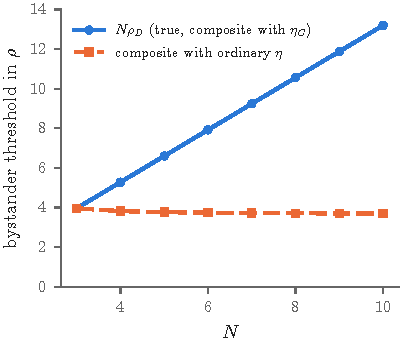
\includegraphics[width=\textwidth]{fig4a_composite_threshold.pdf}
\caption{Bystander threshold}
\end{subfigure}\hfill
\begin{subfigure}[t]{0.45\textwidth}\centering
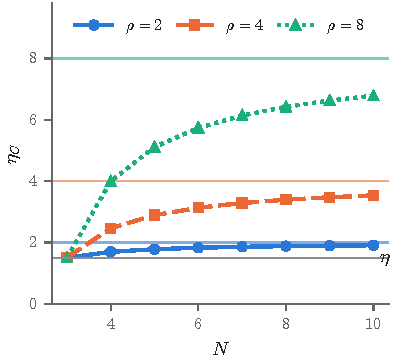
\includegraphics[width=\textwidth]{fig4b_eta_C.pdf}
\caption{Effective elasticity $\eta_C$}
\end{subfigure}
\caption{The composite bystander, US-like parameters. (a) The true threshold $N\rho_D$ for $N=3,\dots,10$, which the composite with $\eta_C$ reproduces exactly, and the threshold of the ``ordinary-$\eta$'' composite, which is nearly flat and slightly declining. (b) $\eta_C$ from \cref{eq:etaC} against $N$ for $\rho\in\{2,4,8\}$, converging toward $\rho$ (thin horizontal lines); the grey line is $\eta=1.5$.}
\label{fig:composite}
\end{figure}

\subsection{Real exchange rates}
\label{sec:real}

Real rates add a price-index wedge: the tariff raises $A$'s consumer prices directly. With $\bar t$ the average tariff and partners imposing no tariffs,
\begin{equation}
d\log q_{Aj}=\Big(1-\tfrac{mN}{N-1}\Big)d\nu_j-m\bar t,\qquad
dq^E_A=\Big[\Big(1-\tfrac{mN}{N-1}\Big)\lambda_{\mathrm{avg}}-m\Big]\bar t.
\label{eq:real}
\end{equation}

\begin{proposition}[Real exchange rates]
\label{prop:real}
Consider a unilateral tariff at the symmetric benchmark.
\begin{enumerate}[label=(\roman*)]
\item If $m<1/N$ and MML holds at the relevant $\rho$, the real bilateral threshold exceeds the nominal one:
\begin{equation*}
\rho^*_q(N)=\frac{[(N-1)-mN]N\rho_D+mN[N\alpha_D(\eta-1)+1]}{(N-1)(1-mN)}>N\rho_D.
\end{equation*}
\item If $m<(N-1)/N$, the REER appreciates.
\end{enumerate}
\end{proposition}

At US-like parameters and $N=3$, $\rho^*_q=4.93$, against $3\rho_D=3.96$.
